\documentclass[border=4pt]{standalone}

\usepackage{pgfplots}
\usepackage{pgfplotstable}
\pgfplotsset{compat=1.18, width=8.5cm, height=5.6cm, tick label style={font=\small}, label style={font=\small}, legend cell align=left, legend style={font=\small, draw=none, fill=none}}
\usepgfplotslibrary{statistics}

\definecolor{plnavy}{HTML}{1F4E89}
\definecolor{plrose}{HTML}{B85A52}
\definecolor{plsage}{HTML}{93CC9E}
\definecolor{plsand}{HTML}{E0BE78}
\definecolor{plplum}{HTML}{8E7BB5}
\definecolor{plgray}{HTML}{6E6E6E}

% ==== data: edit the numbers inside each boxplot prepared={...} below ====

\begin{document}
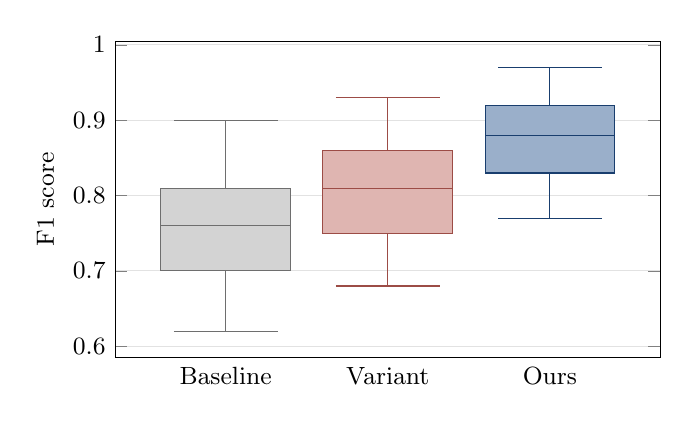
\begin{tikzpicture}
\begin{axis}[boxplot/draw direction=y, ylabel={F1 score}, xtick={1,2,3}, xticklabels={Baseline, Variant, Ours}, xtick style={draw=none}, ymajorgrids, grid style={plgray!20}]
  \addplot[boxplot prepared={lower whisker=0.62, lower quartile=0.70, median=0.76, upper quartile=0.81, upper whisker=0.90}, draw=plgray, fill=plgray!30, solid] coordinates {};
  \addplot[boxplot prepared={lower whisker=0.68, lower quartile=0.75, median=0.81, upper quartile=0.86, upper whisker=0.93}, draw=plrose!85!black, fill=plrose!45, solid] coordinates {};
  \addplot[boxplot prepared={lower whisker=0.77, lower quartile=0.83, median=0.88, upper quartile=0.92, upper whisker=0.97}, draw=plnavy!80!black, fill=plnavy!45, solid] coordinates {};
\end{axis}
\end{tikzpicture}
\end{document}
